% Created 2021-04-06 Tue 10:00
% Intended LaTeX compiler: pdflatex
\documentclass[11pt]{article}
\usepackage[utf8]{inputenc}
\usepackage[T1]{fontenc}
\usepackage{graphicx}
\usepackage{grffile}
\usepackage{longtable}
\usepackage{wrapfig}
\usepackage{rotating}
\usepackage[normalem]{ulem}
\usepackage{amsmath}
\usepackage{textcomp}
\usepackage{amssymb}
\usepackage{capt-of}
\usepackage{hyperref}
\usepackage{minted}

\usepackage{tikz}

% Example dynamics: \p \Cresc \ff
\newcommand{\ppp}{\textbf{\emph{ppp}}}
\newcommand{\pp}{\textbf{\emph{pp}}}
\newcommand{\p}{\textbf{\emph{p}}}
\renewcommand{\mp}{\textbf{\emph{mp}}}
\newcommand{\mf}{\textbf{\emph{mf}}}
\newcommand{\f}{\textbf{\emph{f}}}
\newcommand{\ff}{\textbf{\emph{ff}}}
\newcommand{\fff}{\textbf{\emph{fff}}}

\newcommand{\Cresc}{%
  \vspace{.1em}
  \begin{tikzpicture}
    \draw[line width=1pt] (0.5, 0.1) --  (0, 0) --  (0.5, -0.1)
  \end{tikzpicture}
  \vspace{.3em}}

\newcommand{\Dim}{%
  \vspace{.1em}
  \begin{tikzpicture}
    \draw[line width=1pt] (0, 0.1) --  (0.5, 0) --  (0, -0.1)
  \end{tikzpicture}
  \vspace{.3em}}


% Command to express either bar or rehearsal numbers or letters  
\newcommand{\Boxed}[1]{\fbox{#1} \hspace{0.2 em}}
% \newcommand{\Bar}[1]{{\fbox{#1}}}
% \newcommand{\Boxed}[1]{\fbox{#1}}

\usepackage{harmony}
\author{Torsten Anders}
\date{\today}
\title{TOT Tutorial}
\hypersetup{
 pdfauthor={Torsten Anders},
 pdftitle={TOT Tutorial},
 pdfkeywords={},
 pdfsubject={},
 pdfcreator={Emacs 25.3.50.1 (Org mode 9.2.6)}, 
 pdflang={English}}
\begin{document}

\maketitle
\setcounter{tocdepth}{4}
\tableofcontents


\section{Introduction}
\label{sec:org880776f}

This document presents in a tutorial fashion some functionality of the \href{https://github.com/tanders/tot}{TOT library} for
\href{http://opusmodus.com/}{Opusmodus}. The TOT library is a loose collection of tools for algorithmic composition. This library
implements some features, where a number of definitions work together. This tutorial focusses on
documenting such features. Other functions are self-contained, and their \href{../reference/index.html}{reference documentation}
is probably sufficient.


\textbf{This document is unfinished\ldots{}}


\section{Score processing}
\label{sec:org046319c}

\subsection{Score preview}
\label{sec:org0d241bb}


\subsection{Score transformations}
\label{sec:orga598e42}


\section{Microtonal and xenharmonic music with regular temperaments}
\label{sec:orgd94fd22}

\subsection{Introduction}
\label{sec:org6df8c16}

The TOT library greatly expands Opusmodus' builtin support for microtonal music.  Opusmodus'
builtin support for microtonal music only allows for quarter tones (24 tone equal division of
the octave, 24-EDO) and eighth tones (48 tone equal division of the octave, 48-EDO). The
microtonal model of the TOT library, by contrast, allows users to define arbitrary equal
temperaments (both equal divisions of the octave and other intervals), just intonation (JI) for
arbitrary prime limits, and arbitrary regular temperaments
(\url{https://en.xen.wiki/w/Tour\_of\_Regular\_Temperaments}). 

The library provides this tuning universe in a way that is controllable by a single uniform
notation embedded in \href{https://opusmodus.com/forums/tutorials/omn-the-language/}{OMN}. Still, the library tries to keep things relatively clear and simple by
introducing mainly one actual new accidental symbol, and that symbol will then be combined with
numbers (for prime limits) to express arbitrary JI pitches, which are then mapped to all the
possible tunings.  Technically, pitch deflections are expressed by OMN articulations, as a
library cannot change the underlying OMN pitch format.

For microtonal playback, the library implements what could be called a subset of \href{https://www.midi.org/midi-articles/midi-polyphonic-expression-mpe}{MIDI Polyphonic
Expression (MPE)}, where chords are distributed automatically over multiple MIDI channels so that
each tone is tuned independently by pitch bend messages. A considerable number of soft synth
already support MPE directly (\href{https://roli.com/mpe}{some incomplete list is shown here, scroll down and select Soft
Synths}), and every instrument plugin can be relatively easily made to support MPE by
using multiple instances of that plugin in parallel (e.g., directly in a DAW or with a plugin
host that itself is also a plugin, like \href{https://www.plogue.com/products/bidule.html}{Plogue Bidule}).


The core idea of this xemharmonic support is that JI, arbitrary equal temperaments and very many
other tunings (\url{https://en.xen.wiki/w/Tour\_of\_Regular\_Temperaments}) can all be expressed as
regular temperaments. You can find an informal discussion of regular temperaments, its context
and motivation -- how it extends/generalises many other tone systems -- at this link:
\url{http://x31eq.com/paradigm.html}. Here is another introduction: \url{https://en.xen.wiki/w/Mike\%27s\_Lectures\_On\_Regular\_Temperament\_Theory}. 


\subsection{First steps}
\label{sec:orgc1e7c9f}

Importantly, regular temperaments can all be mapped to JI. Therefore, they can also all by
notated by a pitch notation capable of notating JI for arbitrary prime limits. So, as a unifying
pitch notation for all these temperaments I am using such a JI notation. Several recent JI staff
notations \footnote{I found so far 5 of such JI notations. Examples of highly developed and more
widely used notations are Sagittal (\url{http://sagittal.org}) and the Helmholtz-Ellis JI Pitch
Notation (\url{https://marsbat.space/pdfs/notation.pdf}).} are based on the same fundamental idea: the
traditional pitch nominals (A, B, C\ldots{}) and the traditional accidentals (sharp, double-sharp,
flat\ldots{}) are denoting tones in a Pythagorean tuning (when the notation is read as a JI
notation), i.e. the traditional nominals and accidentals notate all the pitches we can reach
when stacking just fifths (plus their octaves). The core idea of these JI pitch notations is
that they introduce a new accidental for the comma (\url{https://en.wikipedia.org/wiki/Comma\_(music)})
of every prime limit (\url{https://en.wikipedia.org/wiki/Limit\_(music)}). These notations
mainly differ in what kind of symbols they propose for these comma-accidentals.

The JI notation of this library is based on the same principle idea. We notate Pythagorean
nominals and accidentals using the standard OMN pitch notation. Here is a dominant seventh
chord, which in a JI interpretation would be tuned in Pythagorean tuning.

\begin{minted}[]{lisp}
(setf pythagorean-seventh '(h c4e4g4bb4))
\end{minted}


We can play this chord in JI with the TOT macro \texttt{def-tempered-score}. This macro does almost
exactly what the Opusmodus builtin \texttt{def-score} does, but it additionally receives a temperament as
one of its arguments. Also, there are multiple MIDI channels specified per instrument, as
simultaneous tones are played on different MIDI channels, so they can be tuned individually by
pitch bend (the macro uses the \texttt{def-score} tuning argument in the background). Only chords with as
many tones as we specify MIDI channels can be independently/correctly tuned.

\begin{minted}[]{lisp}
(def-tempered-score my-score-name
    (:temperament '31-limit-JI
     :time-signature '(4 4))
  (instr1
   :omn pythagorean-seventh
   :channel '(1 2 3 4)
   :sound 'gm))
\end{minted}


While \texttt{def-tempered-score} generates the score, it does not actually display it nor play it back
(the built-in \texttt{def-score} behaves in the same way). We can always play back and notate the last
score explicitly with the next code snippet. The notation also reveals how \texttt{def-tempered-score}
works in the background: it splits the given score instrument (\texttt{instr1}) with the chord into as
many staves as there are MIDI channels, so that these resulting monophonic staves can be
independently tuned via MIDI pitchbend.

\begin{minted}[]{lisp}
(audition-last-score)
(display-musicxml *last-score* :display :window)
\end{minted}

\begin{figure}[htbp]
\centering
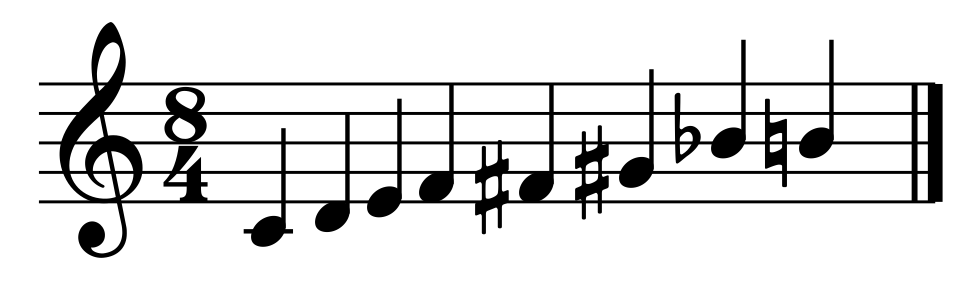
\includegraphics[angle=90,width=5cm]{./graphics/test2.png}
\caption{Some TMP test image}
\end{figure}


Instead of first defining a score with \texttt{def-tempered-score} and then explicitly triggering
its notation or playback as shown, we can also use the TOT function \texttt{preview-score}, which then calls
\texttt{def-tempered-score} in the background. We will commonly use a single temperament and a fixed set
of instruments when working on a piece, so we might want to specify their settings only once and
then use it for notating and playing back multiple snippets.

We can set the tuning separately using the variable \texttt{*current-temperament*}.

\begin{minted}[]{lisp}
(setf *current-temperament* '31-limit-JI)
\end{minted}

We can specify all other score settings via the two variables \texttt{*default-preview-score-header*} and
\texttt{*default-preview-score-instruments*}, where \texttt{*default-preview-score-header*} is a keyword list
(plist) supporting all keyword arguments of \texttt{def-score}.

\begin{minted}[]{lisp}
(setf *default-preview-score-header*
      '(:title "Dummy title"
	:tempo 80))
\end{minted}

Any instrument-specific settings can be specified with the variable
\texttt{*default-preview-score-instruments*} for each instrument we want to use. The instrument labels we
use here are the same that we will later use in the score short-hand format given to
\texttt{preview-score}. Note that multiple MIDI channels are specified here again, and also note the
nested quote (\texttt{'}) signs.

\begin{minted}[]{lisp}
(setf *default-preview-score-instruments*
      '(:instr1 (:sound 'gm
		 :channel '(1 2 3 4))))
\end{minted}

We can now instead of \texttt{def-tempered-score} use the shorter call \texttt{preview-score} with these
settings. The function \texttt{preview-score} is designed for playing back polyphonic scores, so we need
to specify the instrument labels as well.

\begin{minted}[]{lisp}
(preview-score (list :instr1 pythagorean-seventh))
\end{minted}


OK, how about instead of the Pythagorean third we want to use a just major third -- and also a
harmonic seventh and the 11ths overtone? All pitches that go beyond Pythagorean tuning are
notated using JI accidentals that express microtonal comma inflections. 

I suggest we use the letter \texttt{K} for marking any OMN attribute that serves as a Komma
accidental,\footnote{Our letter \texttt{K} is similar to the Greek letter kappa, from where the word comma
comes. (Besides, the letter \texttt{C} is already used in OMN for cent values). When extending OMN as
users by microtonal accidentals, we are restricted to plain ASCII letters and numbers. Most of the
ASCII special characters are already used for something else in OMN and are therefore unavailable
for accidental symbols. Also, while the underlying CCL compiler does support unicode, unicode
support in OMN attribute names is currently limited. I could use greek letters in the names of
custon OMN attributes, but all unicode symbols I tried -- e.g., any mathematical symbols or arrows
-- were not supported. Anyway, while such characters could currently not be used for the attribute
name, they can be used for the string that is then shown for the attribute in the score.} and then
to simply complement that letter with the digits of the prime of the comma in question. So, the
OMN accidental for the \href{https://en.wikipedia.org/wiki/Syntonic\_comma}{5-limit comma (the syntonic comma)} is notated \texttt{5K}, the \href{https://en.wikipedia.org/wiki/Septimal\_comma }{7-limit comma} is
notated \texttt{7K} and so forth. These accidentals raise the pitch by that comma. For a comma flat, put
a minus in front of the accidental, e.g., \texttt{-5K}. So, here is how we can notate and play\footnote{Unfortunately, we cannot yet define new shortcuts for the standard Opusmodus editor. I am instead
using Opusmodus mainly with Emacs, and I defined a shortcut for me for such microtonal snippets
that calls the TOT function \texttt{prevew-score}, which in turn calls \texttt{def-tempered-score} with the OMN
expression before the cursor.} the just harmonic seventh chord.  \texttt{1K} is the natural sign, and
multiple accidental attributes for a chord are assigned in ascending order of chord tones.


\begin{minted}[]{lisp}
(preview-score (list :instr1 '(h c4e4g4bb4 1K+-5K+1K+-7K)))
\end{minted}


JI leads to an infinite number of different pitches. Temperaments reduce that number. So, how about
we want to play the above chord in, say, 22-tone equal temperament
(\url{https://en.xen.wiki/w/22edo}). We only need to define that temperament. Each regular
temperament (including all equal temperaments and also JI) is specified by only two settings: a small
number of generator intervals, and a val for each generator. The vals together specify how each
prime (up to the prime limit of the temperament) it is mapped to JI. These details are explained
in the next section. For now, the following code simply shows the definition of 22-EDO, which is pretty brief. 

\begin{minted}[]{lisp}
(deftemperament 7-limit-22-EDO
    ;; List of vals
    (list (list 22
		(+ 13 22)
		(+ 7 (* 2 22))
		(+ 18 (* 2 22))))
  ;; List of generators
  (list (/ 1200.0 22)))

(setf *current-temperament* '7-limit-22-EDO)
\end{minted}

After we defined 22-EDO this way, we can play the above chord (and any other 7-limit OMN
intervals) in this temperament.


\begin{minted}[]{lisp}
(preview-score (list :instr1 '(h c4e4g4bb4 1K+-5K+1K+-7K)))
\end{minted}



\subsection{Defining temperaments and scales}
\label{sec:org1bb9c31}

We can define arbitrary regular temperaments simply by specifying their vals and generators. This
section briefly introduces these concept, so that you can define your own temperaments. We will
first define the temperament for 12-tone equal temperament (12-EDO), because that is most widely
used and best understood by most Western musicians. 

All pitches of a regular temperament are specified by a small number of \emph{generators}. For an
equal temperament like 12-EDO, we only need a single generator. We can use the semitone of this
temperament as its generator. All tones of the temperament 12-EDO can then be derived by
stacking that interval multiple times. The semitone of 12-EDO and thus our generator is tuned to
100 \href{https://en.wikipedia.org/wiki/Cent\_(music)}{cents}.

The \href{https://en.xen.wiki/w/Val}{\emph{vals}} of a temperament specify how the intervals of the prime frequency ratios 2, 3,
5\ldots{} up to the prime limit of our temperament are mapped to intervals in this temperament. 

\textbf{TODO}


\begin{minted}[]{lisp}
(deftemperament 11-limit-12-EDO
    (list (edo-val 12 '(0 7 4 10 6)))
  '(100.0)
  "12-EDO temperament with an 11-limit mapping.")
\end{minted}


\subsection{Obtaining information}
\label{sec:org6a04364}

\subsubsection{Information on intervals}
\label{sec:org90cc0ff}


\subsubsection{Information on scales}
\label{sec:org6b6128e}


\subsection{Defining harmony}
\label{sec:orgfbd410f}


\subsection{Constraining music to an underlying harmony}
\label{sec:org2d4f13c}



\subsection{Dynamic temperaments}
\label{sec:orgd674fed}

At a later stage, the library is also meant to support dynamic temperaments, so that the tuning
can change during the course of a piece, but the implementation of dynamic temperaments is
still unfinished.



\section{Form}
\label{sec:orgbd427d6}

\texttt{fn-unfold} 



\section{Karnatic rhythms}
\label{sec:orga2aa36e}

\subsection{Creating a higher-level plan}
\label{sec:orgc321911}


\subsection{Filling in details}
\label{sec:org660cd46}
\end{document}